 ~\vspace{.1in}
 
\section{Rate of change}

A diver bounces on a 3-meter springboard. Up she goes.  A somersault, a twist, then whoosh, into the water.  
The table shows the diver's height as a function of time, 

\begin{center}
\begin{tabular} {|c| | c|c|c|  c|c|c| c|c|} \hline
$T$ & 0 & .2 & .4 & .6 & .8 & 1.0 & 1.2 & 1.4 \\ \hline
$H$ & 3.00 & 3.88 & 4.38 & 4.48 & 4.20  & 3.52 & 2.45 & 1.00 \\ \hline
\end{tabular}
\end{center}
where \begin{center}
\begin{tabular} {l}
$H=$ diver's height (meters) $\sim$ dep \\
$T= $ time (seconds) $\sim$ indep \\ 
\end{tabular}
\end{center}

In case you're wondering, 3 meters is nearly 10 feet up and the highest height listed, 4.48 meters, is close to 15 feet above the water.  More on how we figured those numbers out in the next section, but thought you might like to know.  

How fast is she moving?  The diver starts at 3 meters, which is the height of the springboard, and .2 seconds later she's up to 3.88 meters.  That means during the first .2 seconds, the diver went up $$3.88-3 = .88 \text{ meters}$$
Her speed is  $$\frac{.88 \text{ meters}}{.2 \text{ seconds}} = 0.88 \div .2 = 4.4 \text{ meters/sec}$$

What about during the next .2 seconds?  Does she move faster, slower, or the same?  During this time, her height changed from 3.88 meters to 4.38 meters.  In these .2 seconds she rose $$4.38-3.88 = .50 \text{ meters}$$
That's less than before (since $.50 < .88$), which means so she is going slower.  Let's double check by calculating her speed.
$$\frac{.50 \text{ meters}}{.2 \text{ seconds}} = .50 \div .2 = 2.5 \text{ meters/sec}$$
Yup, slower.

Let's take a look at this calculation again.  Here's what we did.
$$\text{speed} =  \frac{4.38-3.88 \text{ meters}}{.4-.2 \text{ seconds}} = \frac{.50 \text{ meters}}{.2 \text{ seconds}} = .50 \div .2 = 2.5 \text{ meters/sec}$$
There is a way to do the entire calculation at once on your calculator.
$$(4.38-3.88) \div (.4-.2)=2.5 \text{ meters/sec}$$
See how we put parentheses around both the top and bottom of the fraction?  We needed them to force the calculator to do the subtractions first and division second. The usual order of operations would do it the other way around:  multiplication and division before addition and subtraction.  (If you need a reminder, the full list of the order of operations appears later, in Section 1.5.)  Because the top and bottom of the fraction each have meaning in the story, we continue to calculate them separately, but feel free to do the whole calculation at once if you prefer.

Notice that we are subtracting \textbf{like terms}:  meters from meters and then seconds from seconds.  It would not make sense to  mix.  Think:  $$\text{children} -  \text{cookies} = \text{crying}$$
so we don't want to mix units because that would be like taking cookies away from children.

In our story, we calculated the speed of the diver.  In general, that number is the \textbf{rate of change} of the function over that interval of values.  

\bigskip
 \framebox{
 \begin{minipage}[c]{.85\textwidth}  
~ \bigskip \\  \textsc{Rate of change formula:} \quad $ \displaystyle \text{rate of change = }\frac{\text{change dep}}{\text{change indep}}$\\ ~ \bigskip
\end{minipage}
}
\bigskip

\noindent Notice how the change in dependent variable (height, in meters) is on top of the fraction and the change in independent variable (time, in seconds) is on the bottom.  That makes sense in our example because speed is measured in meters/second.  The units can help you keep that straight.
$$\text{units for rate of change} = \frac{\text{units for dep}}{\text{units for indep}}$$

Back to our diver.  During the next time interval she's moving even slower.  
$$\text{speed} = \frac{4.48-4.38 \text{ meters}}{.6-.4 \text{ seconds}}= \frac{.1 \text{ meters}}{.2 \text{ seconds}} = .1 \div .2 = .5 \text{ meters/sec.}$$  
And look what happens when we calculate her speed during the next time interval.  
$$\text{speed} = \frac{4.20-4.48 \text{ meters}}{.8-.6 \text{ seconds}} =  \frac{-.28 \text{ meters}}{.2 \text{ seconds}} = \text{(-)}.28 \div .2 = -1.4 \text{ meters/sec}$$  What does a negative speed mean?  During this time interval her height drops.  She's headed down towards the water.  Her speed is 1.4 meters/sec downward.  The negative tells us her height is falling.  What goes up, must come down.  Sure enough.

You may notice that the signs for subtraction and negation each look like $-$.  On the calculator these are two different keys.  The subtraction key reads just $-$.  The negation key often reads \text{(-)} and is done before the number.  This does not mean you type in parentheses, just hit the one key that is labeled \text{(-)} already.  
(If your calculator does not have a key labeled (-), look for a key labeled $\text{+/-}$ instead.   That is not three keys, just one labeled $\text{+/-}$ Often that key needs to follow the number, so enter 
$$.28\text{ +/- } \div .2 =$$
You should get  -1.4 meters/sec again.)

Here are the speeds included in our table.  
\begin{center}
\begin{tabular} {|c| | c|c|c|  c|c|c| c|c|} \hline
$T$ & 0 & .2 & .4 & .6 & .8 &1.0 & 1.2  &1.4 \\ \hline
$H$ & 3 & 3.88 & 4.38 & 4.48 & 4.20  & 3.52 & 2.45 & 1 \\ \hline
Speed && $\to$ 4.4 & $\to$ 2.5 & $\to$ .5 & $\to$ -1.4 & $\to$ -3.4 & $\to$ -5.35 & $\to$ -7.25  \\ \hline
\end{tabular}
\end{center}

Let's graph our function. Notice that time is on the horizontal axis because it's the independent variable and height is on the vertical axis because it's our dependent variable:  height depends on time.  
\begin{center}
\scalebox {.9} {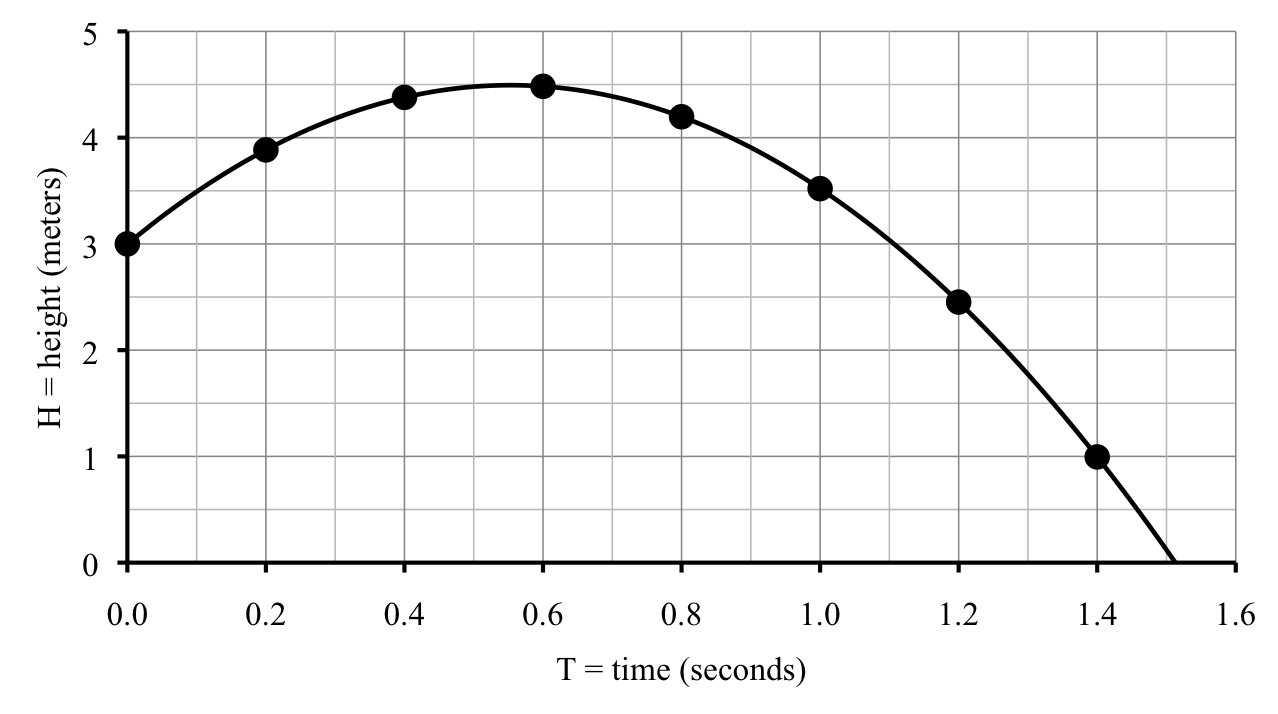
\includegraphics [width = 6in] {springboard_diver.png}}
\end{center}
As usual we drew in a smooth curve connecting the points, which illustrates our best guesses for the points we don't know and we continued the graph until the height was zero (when the diver hits the water).  The values from our table are indicated with big points to help explain what's going on.     

There is a way to see the rate of change from the graph.  In the case of our diver, the graph looks like a hill.  The curve goes uphill at first.  Between the first two points it is rather  steep and the rate of change is 4.4 meters/sec there.  The next segment is less steep and that's where the rate of change is less, down to 2.5 meters/sec.  The third line segment is almost flat and that's where the rate of change is only 0.5 meters/sec.  Aha.  The rate of change corresponds to how steep the curve is. 

We notice the same connection between the rate of change and steepness of the curve for the downhill portion, only this time all the rates of change are negative.  The first downhill segment is not very steep and the rate of change is -1.4 meters/sec there.  The next downhill segment has rate of change -3.4 meters/sec and the graph is steeper.  The next two downhill segments are steeper and steeper yet and this time with rates of change -5.35 and -7.25 meters/sec.

A little more vocabulary here.  For the uphill portion of the graph, from 0 to just before .6 seconds, the rate of change is positive.  The function is \textbf{increasing} there:  as the independent variable gets larger, so does the dependent variable. After about .6 seconds, the graph is downhill and the rate of change is negative.  The function is  \textbf{decreasing} there:  as the independent variable gets larger, the dependent variable gets smaller.

When does the diver's height stop increasing and start decreasing?  When she's at the highest height, some time just before .6 seconds into her dive.  Before then her rate of change is positive.  After that time her rate of change is negative.  So, at the highest height her rate of change is probably equal to zero.  Does that make sense?  Think about watching a diver on film in very slow motion.  Up, up she goes, then almost a pause at the top, and then down, down, into the water.  At the top of her dive it's as if she stands still for an instant.  That would correspond to zero speed.

%\section{Rate of change}

 \begin{center}
\line(1,0){300} %\line(1,0){250}
\end{center}

\section*{Homework}

\noindent \textbf{Start by doing Practice exercises \#1-4 in the workbook.}

\bigskip

\noindent \textbf{Do you know \ldots}

\begin{itemize}
\item How to calculate rate of change between two points?   \emph{Ask your instructor if you need to remember the formula or if it will be provided during the exam.} 
\item What the rate of change means in the story?   
\item How we can use the rate of change to estimate values?   
\item When a function is increasing or decreasing, and the connection to the rate of change?   
\item Why the rate of change is zero at the maximum (or minimum) value of a function?   
\item What the connection is between rate of change and the steepness of the graph?   
\item[~] \textbf{If you're not sure, work the rest of exercises and then return to these questions.  Or, ask your instructor or a classmate for help.} 
\end{itemize}

\subsection*{Exercises}

\begin{enumerate} 
\setcounter{enumi}{4}
\item Look back at the springboard diver example in this section. 
\begin{enumerate}
\item  Check the other rates of change given in the table.
\item Approximately how fast is the diver moving as she enters the water?  Use that her height at 1.4 seconds is 1 foot above water (given earlier), but also her height at 1.5 seconds is just .12 feet above water.
\end{enumerate}

\item Your local truck rental agency lists what it costs to rent a truck (for one day) based on the number of miles you drive the truck.  
\begin{center}
\begin{tabular} {|l| |c |c|c|c|} \hline
Distance driven (miles) & 50 & 100 & 150 & 200 \\ \hline
Rental cost (\$) & 37.50 & 55.00 & 72.50 & 90.00 \\ \hline
\end{tabular}
\end{center}
 \hfill \emph{Story also appears in 1.2 and 4.4 Exercises}
\begin{enumerate}
\item Calculate the rate of change for each time period.
\item Can you use figure out what it probably costs to rent a truck to drive 75 miles?
\item There must be some sort of fixed price plus a per mile price.  Can you figure out what that fixed price must be?  
\end{enumerate}

\item Wind turbines are used to generate electricity.  A few values are recorded in the table
\begin{center}
\begin{tabular} {|c| |c |c|c |c|}\hline
wind speed (mph) & 0 & 10 & 20 & 30 \\ \hline
electricity (watts) & 0 & \text{2,400} & \text{19,200} & \text{64,800} \\ \hline
\end{tabular}
\end{center}
\hfill \emph{Story also appears in 1.1, 2.4, and 3.3 Exercises}

\begin{enumerate}
\item Name the variables, including units and dependence.
\item Plot the points from the table on a graph.
\item Calculate the rate of change in electricity as a function of wind speeds from 0 to 10 mph.  Sketch in the line segment connecting those two points on the graph.   
\item Repeat for wind speeds from 10 to 20 mph.  Is the electricity produced increasing faster or increasing slower than for lower wind speeds.
\item Repeat for wind speeds from 20 to 30 mph.  Comment again on how the rate of change compares to earlier rates of change.
\end{enumerate} 

\item The table lists estimates of Earth's population, in billions, for select years since 1800.   
\begin{center}
\begin{tabular} {|l |c |c |c |c |c |c |c |} \hline
year & 1800 & 1850 & 1900 & 1950 & 1970 & 1990 & 2000 \\ \hline
population & .98 & 1.26 & 1.65 & 2.52 & 3.70 & 5.27 & 6.06  \\ \hline
\end{tabular}
\end{center}
\hfill \begin{footnotesize} Source:  ``The World at Six Billion'' United Nations report, 1999\end{footnotesize}
%http://www.un.org/esa/population/publications/sixbillion/sixbilpart1.pdf

\hfill \emph{Story also appears in 1.2 Exercises}

During which period of time was the Earth's population increasing the fastest?  Calculate the rates of change for each time period to decide.  (Or, explain some other way of deciding.)

\item A company produces backpacks.  The more they make, the less it costs for each one.   For example, if they produce 10 backpack it would cost \$39 each.  For 40 backpacks, they would cost \$18 each.  By 70 backpacks, the unit cost is down to \$15 each.  At 100 backpacks, the unit cost is \$30 each. \hfill \emph{Story also appears in 3.5 Exercises}
\begin{enumerate}
\item Name the variables and summarize the information in a table.
\item Calculate the rates of change between 10 and 40 backpacks, between 40 and 70 backpacks, and between 70 and 100 backpacks.
\item For which range of values does the cost per backpack decrease?  
\item Any ideas why the cost might increase?
\item Draw a graph illustrating the dependence.  Try for a nice, smooth curve.
\item Approximately how many backpacks does the company have to make to keep the cost per backpack as small as possible?
\end{enumerate}

\item The public beach near Paloma's house has lost depth (measured from the dunes to the high water mark) due to erosion since they started keeping records 60 years ago.  The table shows a few values. There $D$ is the depth of the beach in feet, and $Y$ is the year, measured since 60 years ago.  
\begin{center}
\begin{tabular} {|c| |c|c |c |c|}\hline
year & 60 years ago & 30 years ago & 10 years ago & ~\quad now \quad ~\\ \hline
$Y$ & 0 & 30 & 50 & 60 \\ \hline
$D$ & 435 & 322.5 & 247.5 & 210 \\ \hline
\end{tabular}
\end{center} 
\hfill \emph{Story also appears in 4.3 Exercises}
  
\begin{enumerate}
\item Calculate the rates of change for each time period.  
\item Explain why the rates of change should be negative.
\item Approximately how many feet a year is the beach eroding?  
\item Draw a graph showing how the beach depth has changed over the past 60 years.
\end{enumerate}

\end{enumerate}

